%\documentclass[preprint,tightenlines,showpacs,showkeys,floatfix,
%nofootinbib,superscriptaddress,fleqn]{revtex4} 
\documentclass[APS,floatfix,nofootinbib,superscriptaddress,fleqn,preprint]{revtex4} 
%\documentclass[aps,epsfig,tightlines,fleqn]{revtex4}
\usepackage[utf]{kotex}
\usepackage[HWP]{dhucs-interword}
\usepackage[dvips]{color}
\usepackage{graphicx}
\usepackage{bm}
%\usepackage{fancyhdr}
%\usepackage{dcolumn}
\usepackage{defcolor}
\usepackage{amsmath}
\usepackage{amsfonts}
\usepackage{amssymb}
\usepackage{amscd}
\usepackage{amsthm}
\usepackage[utf8]{inputenc}
 \usepackage{setspace}
%\pagestyle{fancy}

\begin{document}

\title{\Large 2022년 1학기 물리학 I: Quiz 2}
\author{김현철\footnote{Office: 5S-436D (면담시간 매주s
    화요일-16:00$\sim$20:00)}} 
\email{hchkim@inha.ac.kr}
\author{Hui-Jae Lee} 
\email{hjlee6674@inha.edu}
\affiliation{Hadron Theory Group, Department of Physics, Inha University,
Incheon 402-751, Republic of Korea }
\date{Spring semester, 2022}


\vspace{1.cm}
\begin{abstract}
\noindent \textbf{ {\color{red}주의}: \color{blue} 단 한 번의 부정행위도 절대
  용납하지 않습니다. 적발 시, 학점은 F를 받게 됨은 물론이고,
  징계위원회에 회부합니다. One strike out임을 명심하세요.}\\
\\
문제는 다음 쪽부터 나옵니다.  \\ \\
{\bf Date:} 2022년 3월 7일 (월) 15:30-16:15 
\\
{\bf 학번:} \hspace{4cm}
{\bf 이름:} 

\end{abstract}
\maketitle

\noindent {\bf 문제 1 [20pt]}
그림~\ref{fig:1}과 같이 크기가 각각 1, 2, 4인 세 벡터 $\vec{A}$,
$\vec{B}$, $\vec{C}$가 같은 평면상에 놓여 있다. 벡터 $\vec{A}$와 벡터
$\vec{B}$는 서로 수직이고, 벡터 $\vec{B}$와 벡터 $\vec{C}$의 끼인각이 30°일 때,
벡터 $\vec{C}$는 벡터 $\vec{A}$와 벡터 $\vec{B}$를 사용하여
\begin{align*}
\vec{C} = \alpha \vec{A} + \beta\vec{B}  
\end{align*}
로 나타낼 수 있다. 두 상수 $\alpha$와 $\beta$를 구하여라. 
\begin{figure}[ht]
  \centering
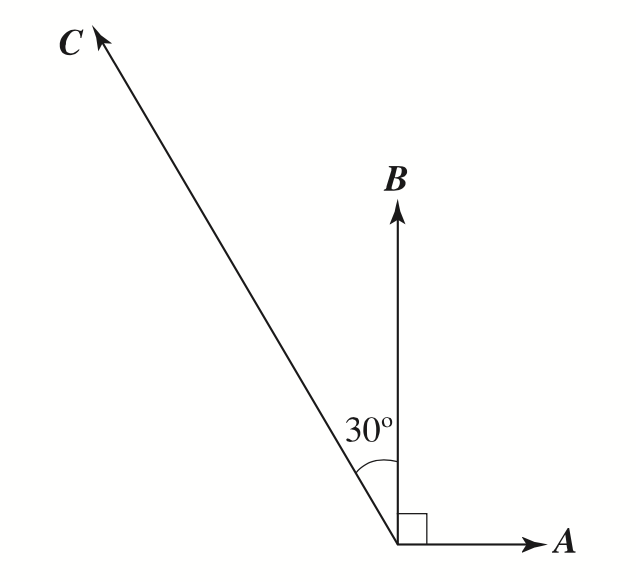
\includegraphics[scale=0.6]{Qfig3-1-20220307.png}  
  \caption{문제 1}
  \label{fig:1}
\end{figure} 

\noindent {\bf 해답} $\vec{A}$ 와 $\vec{B}$ 가 서로 수직이므로, $\vec{A} \cdot \vec{B} =0 $ 이다. 이는 다음을 의미한다.
\begin{align*}
  \vec{C} \cdot \vec{A} =\alpha\, \quad
  \vec{C} \cdot \vec{B} =\beta 
\end{align*}
스칼라곱의 정의를 이용하면 $\alpha$ 와 $\beta$ 를 구할 수 있다. 스칼라곱의 정의는 다음과 같다.
\begin{align*}
  \vec{A} \cdot \vec{B} = |\vec{A}||\vec{B}|\cos{\theta}
\end{align*}
이로부터 $\alpha$ 와 $\beta$ 는 다음과 같이 표현이 가능하다.
\begin{align*}
  \alpha &= |\vec{C}||\vec{A}|\cos{120^{\circ}} = 4 \times \left(-\frac{1}{2}\right) = -2 \\
  \beta &= |\vec{C}||\vec{B}|\cos{30^{\circ}} = 4 \times \frac{\sqrt{3}}{2} = 2\sqrt{3}
\end{align*}
따라서, $\vec{C}$ 는 다음과 같다.
\begin{align*}
  \vec{C} = -2 \vec{A} + 2\sqrt{3} \vec{B}
\end{align*}
\newpage

{\color{gray} [문제 풀이 쪽]}

\newpage 

\noindent {\bf 문제 2 [10pt]}
물리학자이자 의사였던 미공군 존 스탭(John P. Stapp) 대령은 제트기에서
조정사가 비상탈출을 했을 때 살아남을 수 있는지 직접 실험을
했다. 1954년 3월 19일, 그는 로켓을 단 차를 선로 위를 달릴 수 있도록
제작한 뒤,  1\,011 km/h의 속력으로 달렸다. 그리고 도착점에 거의 다
도달했을 때, 제동을 걸어 1.40 s만에 멈췄다. 
\begin{figure}[ht]
  \centering
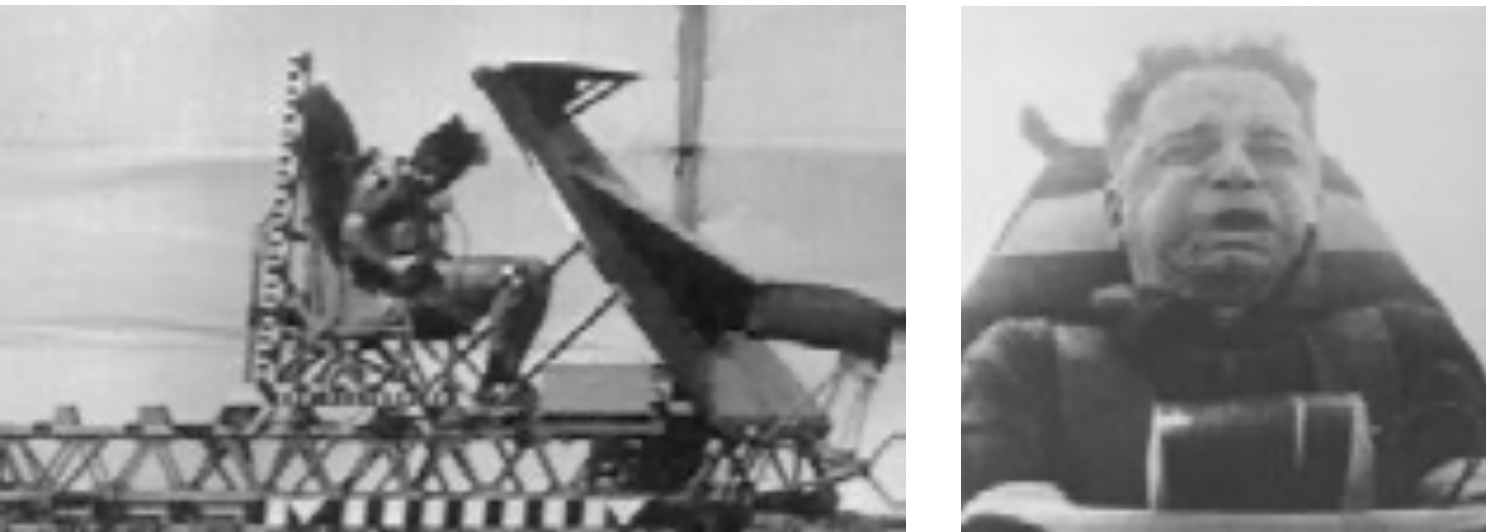
\includegraphics[scale=0.5]{Qfig3-2-20220307.png}  
  \caption{문제 2}
  \label{fig:2}
\end{figure}
\begin{itemize}
\item[(가)] 스탭 대령이 경험한 음의 가속도(감속도)를 구하여라. 구한
  가속도의 크기를 중력가속도 $g=9.80\,\mathrm{m/s^2}$로 나타내어라.
\item[(나)] 이 가속도를 받는 1.4 s  동안 스탭 대령이 간 거리는 얼마인가?
\end{itemize}
(이 실험으로 스탭 대령은 무릎뼈가 골절되고, 눈에 심각한 부상을 입어서
훗날 백내장으로 고생했다고 한다. 이 실험으로 스탭 대령은 자동차에 안전벨트를
도입하는 데 지대한 공을 세웠다.) \\
\noindent {\bf 풀이} 
\begin{itemize}
  \item [(가)] 스탭 대령의 처음 속력은 1\,011 km/h 이고 정지하였으므로, 나중 속력은 0 km/h 이다. 걸린 시간 1.40 s 와 단위 환산을 고려하여 다음과 같이 평균 가속도의 크기를 계산할 수 있다.
  \begin{align}
    a_{avg} = \left(\frac{(0-1\,011)\mathrm{km/h}}{1.40 \,\mathrm{s}}\right)\times\left(\frac{3600\,\mathrm{s}}{1\,\mathrm{h}}\right)=2\,600\,000\,\mathrm{km/h^2}
  \end{align} 
  중력 가속도와 비교하기 위해, 단위를 바꾸어서 표현해보자.
  \begin{align}
    \left(\mathrm{\frac{2\,600\,000\,km}{h^2}}\right)\times\left(\mathrm{\frac{1000\,m}{1\,km}}\right)\times\mathrm{\left(\frac{1\,h}{3\,600\,s}\right)^2}=200\,\mathrm{m/s^2}
  \end{align}
  중력 가속도의 크기를 1\,G 라고 하면, 다음과 같이 표현할 수 있다.
  \begin{align}
  \mathrm{200\,m/s^2}\times\left(\frac{1\,\mathrm{G}}{9.8\,\mathrm{m/s^2}}\right) = 20\,\mathrm{G}
  \end{align} 
  스탭 대령은 감속하면서 중력 가속도의 크기의 20배에 해당하는 가속력을 받았다.
  \item [(나)] 처음 속력과 나중 속력, 평균 가속도를 알고 있으므로, 다음의 공식을 이용해 이동한 거리를 구할 수 있다.
  \begin{align}
    v^2=v_0^2+2a_{avg}(x-x_0)
  \end{align}
  나중 속력은 $v=\mathrm{0\,km/h}$, 처음 속력은 $v_0=\mathrm{1\,011\,km/h}$, 평균 가속도의 크기는 $a_{avg}=2\,600\,000\mathrm{km/h^2}$ 이다. 스탭 대령은 감속을 하였으므로, 가속력이 들어가는 항의 부호를 -로 바꿔주어야 한다. 감속을 시작한 지점을 시작점으로 생각하면, $x_0=0\,\mathrm{km}$ 이다. $x$ 를 구해보자.
  \begin{align}
    0=\left(\mathrm{1\,011\,km/h}\right)^2-2\times\left(2\,600\,000\mathrm{km/h^2}\right)\times x
  \end{align}    
  편한 계산을 위해, 구하고자 하는 값을 제외한 모든 값을 반대쪽으로 넘기자.
  \begin{align}    
    x=\frac{\left(\mathrm{1\,011\,km/h}\right)^2}{2\times\left(2\,600\,000\mathrm{km/h^2}\right)}=0.1966\,\mathrm{km}=196.6\,\mathrm{m}
  \end{align}
  스탭 대령은 감속하는 동안, 196.6\,m 만큼 이동했다.
\end{itemize}

\newpage

{\color{gray} [문제 풀이 쪽]}

\newpage 

\noindent {\bf 문제 3 [10pt]} 
어떤 전투기가 그림~\ref{fig:2}에서처럼
35 m의 높이에서 $1\,300$ km/h의 속력으로 수평하게 날고 있다. $t=0$에서
이 전투기는 $\theta=4.3^\circ$의 각도로 기울어져 있는 언덕 위를
비행하기 시작했다. 만일 조종사가 이 전투기의 방향을 바꾸지 않는다면,
이 전투기는 언제 언덕과 충돌하게 되겠는가? 
\begin{figure}[ht]
  \centering
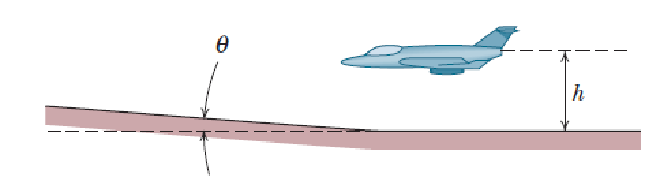
\includegraphics[scale=1.0]{Qfig3-2.pdf}  
  \caption{문제 1}
  \label{fig:1}
\end{figure} \\
\noindent {\bf 풀이} 
전투기가 비행한 거리를 $d(t)$ 라 하고, 전투기가 위치한 언덕의 높이를 $s(t)$ 라 하면, $d$ 와 $s$ 사이에는 다음의 상관관계가 있다.
\begin{align}
  \tan{4.3^\circ} =\frac{s(t)}{d(t)} 
\end{align}
우리는 언덕의 높이가 35m 일 때, 전투기가 비행한 시간을 알고 싶다. 전투기가 등속 직선 운동한다고 가정하면, $d(t)$ 는 다음과 같다.
\begin{align}
  d(t) = \frac{1\,300\,\mathrm{km}}{1\,\mathrm{h}}\times t
\end{align}
식 (7) 에 지금까지의 이야기 한 것들을 대입해보자.
\begin{align}
  &\tan{4.3^\circ} \times \left(\frac{1\,300\,\mathrm{km}}{1\,\mathrm{h}}\right) \times \left(\frac{1\mathrm{h}}{3\,600\,\mathrm{s}}\right) \times \left(\frac{1\,000\,\mathrm{m}}{1\,\mathrm{km}}\right) \times t = 35\,\mathrm{m}
\end{align}
단위를 고려하여 변환하고 구하고자 하는 변수 $t$ 만 좌항에 남기면 다음과 같다.
\begin{align}    
  &0.075\times 360\,\mathrm{m/s}\times t = 35\,\mathrm{m} \\
  &t=35\,\mathrm{m}\times\left(\frac{1\,\mathrm{s}}{360\,\mathrm{m}}\right) \times \left(\frac{1}{0.075}\right) = 1.3\,\mathrm{s}
\end{align}
전투기는 1.3 초 후에 충돌한다.
\newpage

{\color{gray} [문제 풀이 쪽]}

\newpage

\noindent {\bf 문제 4 [20pt]}
공사 중인 다리에서 볼트가 다리 아래 계곡으로 90 m 떨어진다.
\begin{itemize}
\item[(가)] 낙하거리의 마지막 20\% 지나는 데 걸리는 시간을 구하여라.
\item[(나)] 볼트가 낙하거리의 마지막 20\%를 들어설 때의 속력을
  구하여라.
\item[(다)] 다리 아래 계곡에 도달할 때 볼트의 속력을 구하여라.   
\end{itemize}


\newpage

{\color{gray} [문제 풀이 쪽]}

\newpage

\end{document}
